\documentclass[compress]{beamer}
\usepackage{ifthen,verbatim}

\setbeamertemplate{navigation symbols}{}
\setbeamertemplate{headline}{}

\begin{document}

\begin{frame}
\frametitle{Effect of $p_T$ $>$ 100~GeV on alignment}

\begin{itemize}
\item Production alignment used only tracks with \mbox{$20<p_T<100$~GeV\hspace{-2 cm}}
\item Starting from the above, we re-aligned with \mbox{$100<p_T<200$~GeV\hspace{-2 cm}}
\item These are the differences between the low-momentum alignment and the high-momentum alignment
\item \mbox{\scriptsize (Converged after 2 iterations, as expected, and only showing ``$\sigma$'' $<$ 1~mm, 1~mrad)\hspace{-1 cm}}
\end{itemize}

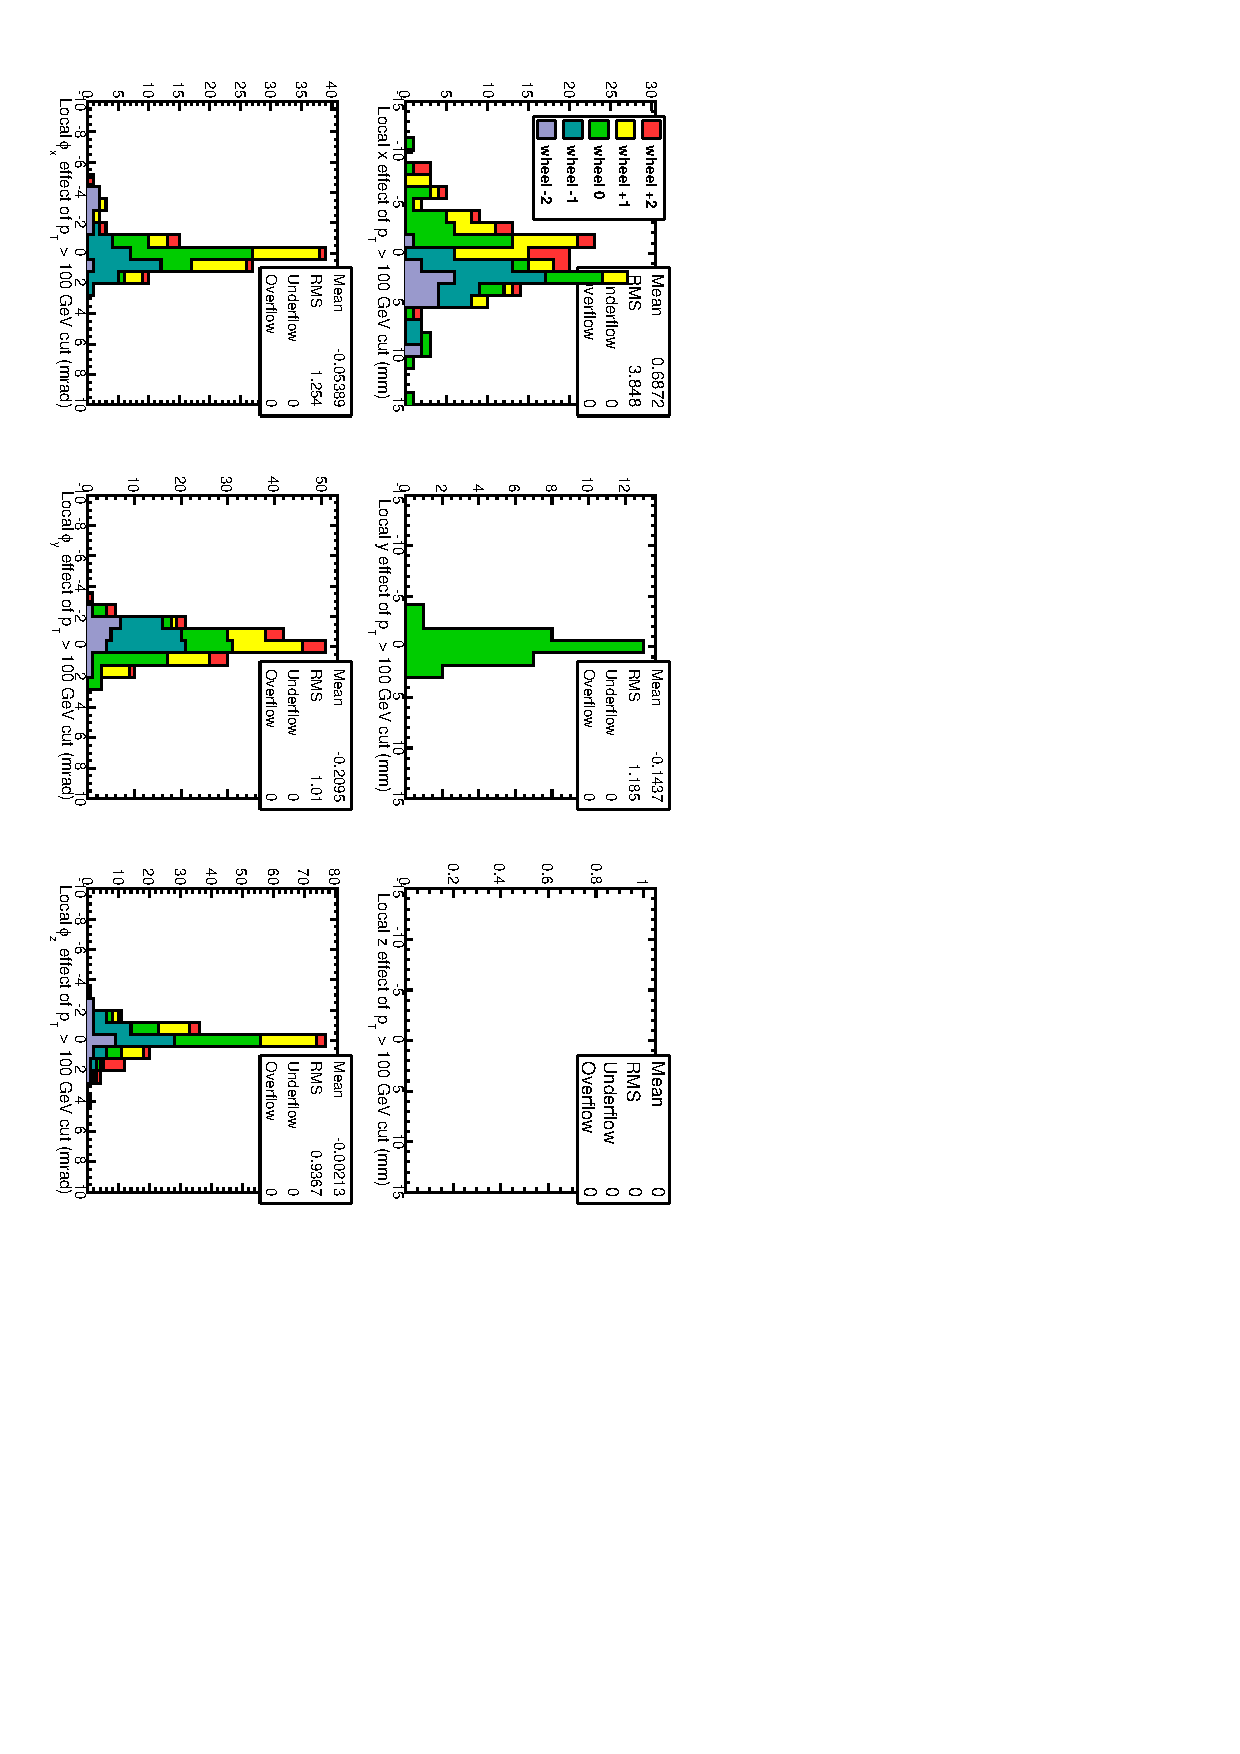
\includegraphics[height=\linewidth, angle=90]{data_effect_of_100GeVcut.pdf}
\end{frame}

\begin{frame}
\frametitle{Effect of $p_T$ $>$ 100~GeV on alignment}

\begin{itemize}
\item Here it is again, split up by station instead of wheel
\item Even though these are 5--10~mm displacements, we {\it have not}
  returned to CRAFT\_ALL\_V4 (before first global alignment).  This is a new configuration.
\end{itemize}

\vfill
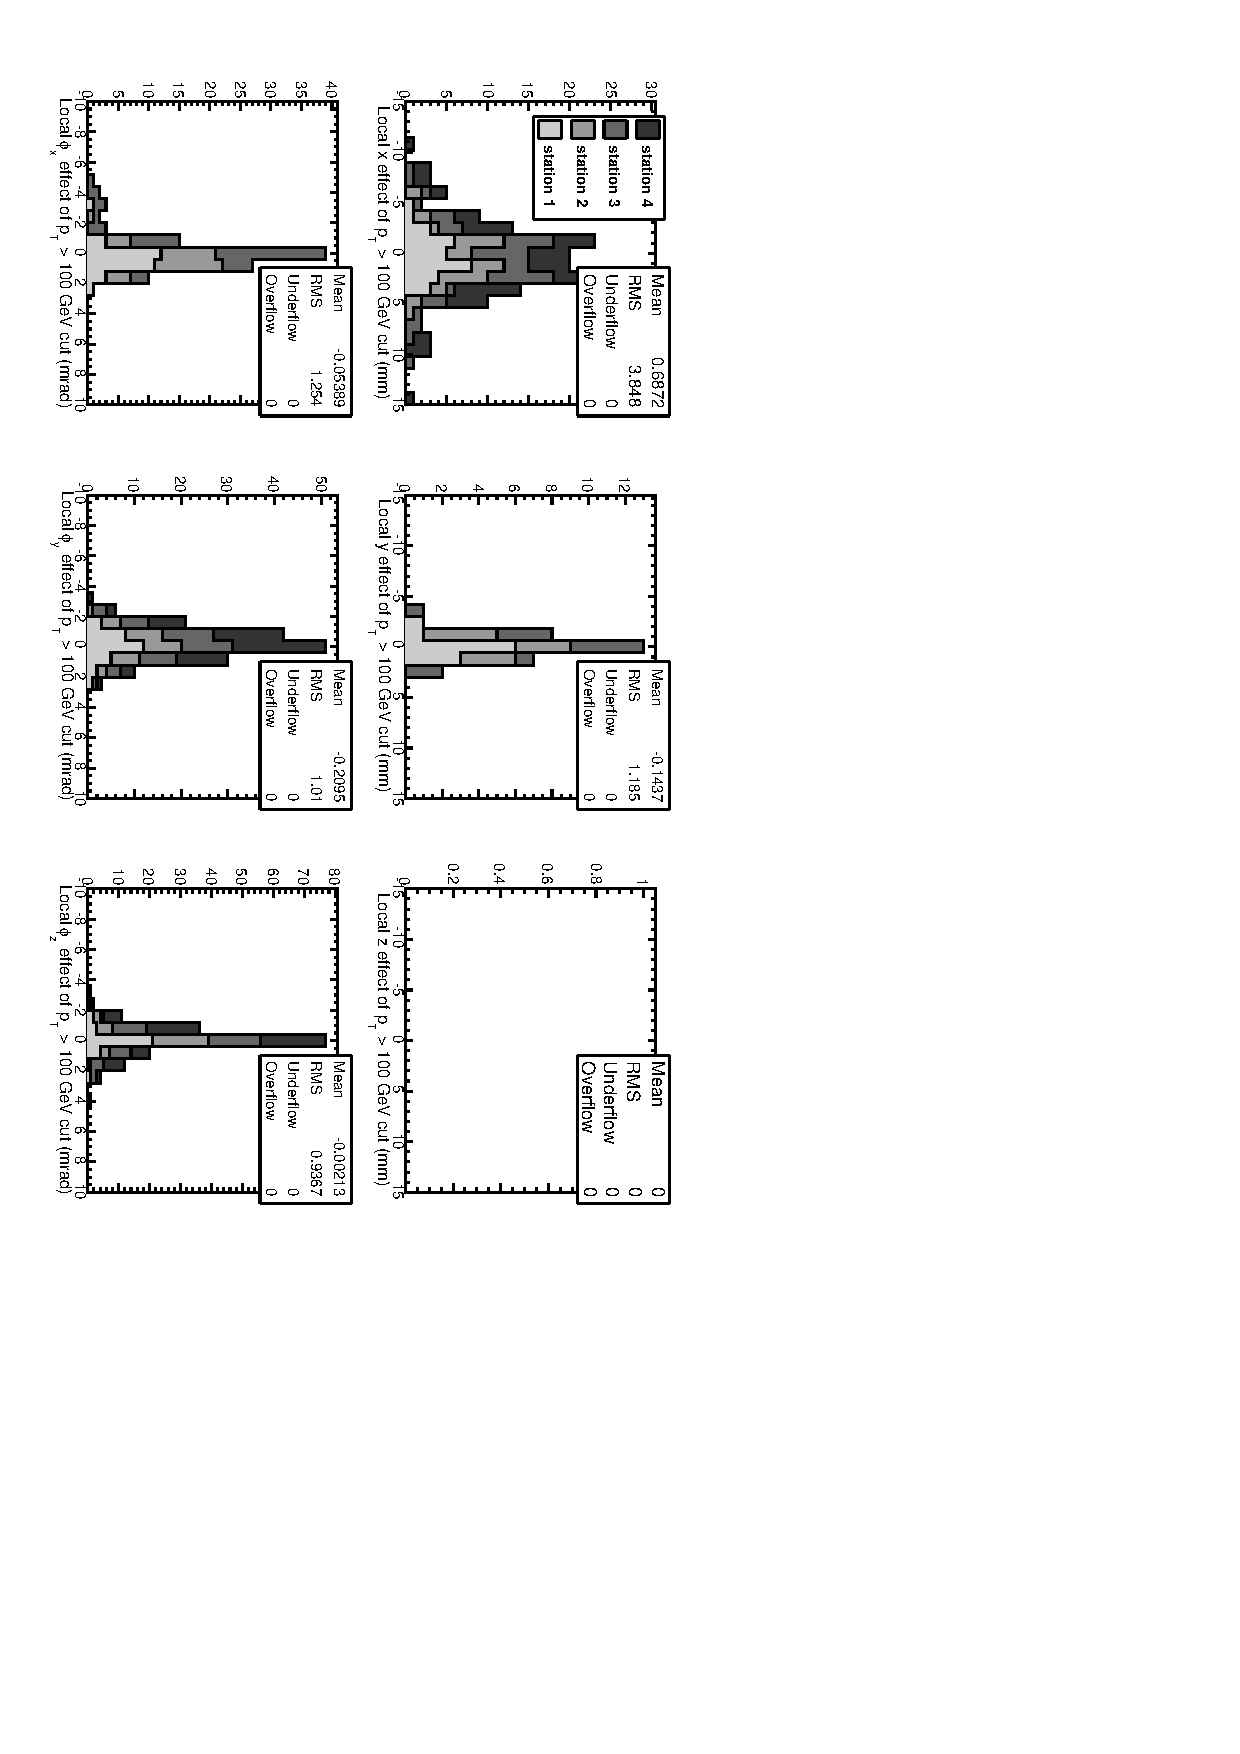
\includegraphics[height=\linewidth, angle=90]{data_effect_of_100GeVcut2.pdf}
\end{frame}

\begin{frame}
\frametitle{Effect of $p_T$ $>$ 100~GeV on alignment}

\begin{itemize}
\item And now in global $\Delta \phi$ around beamline and global $r\phi$
\item Yes, we see a rotation (0.34~mrad) and a twist (0.04~mrad/m)
\item But it is a $p_T$-dependent effect--- rotation {\it relative to low-$p_T$!}
\item Hypothesis: curl in tracker causes $p_T$-dependent apparent rotation in the other direction (spread could be statistical)
\end{itemize}

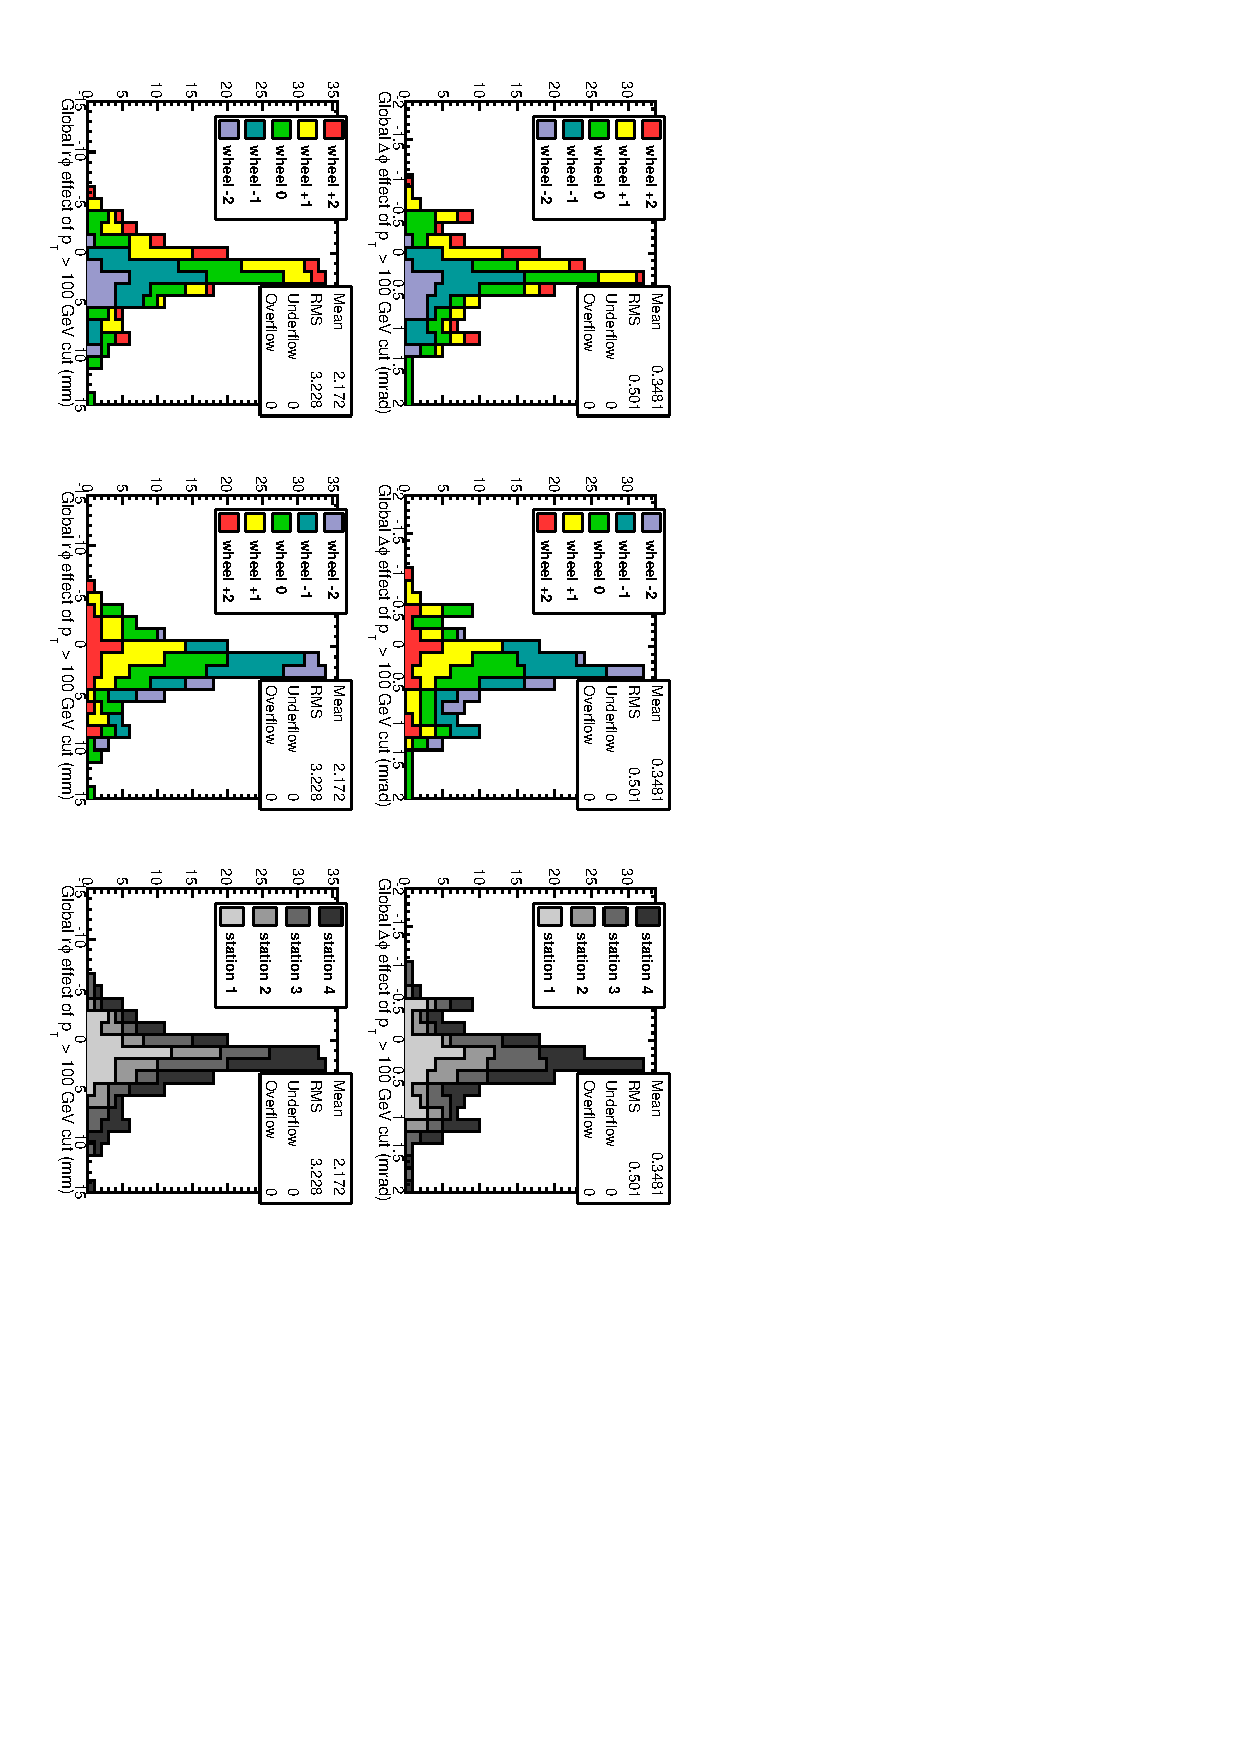
\includegraphics[height=\linewidth, angle=90]{data_effect_of_100GeVcut3.pdf}
\end{frame}

\begin{frame}
\frametitle{Diagram of curl hypothesis}

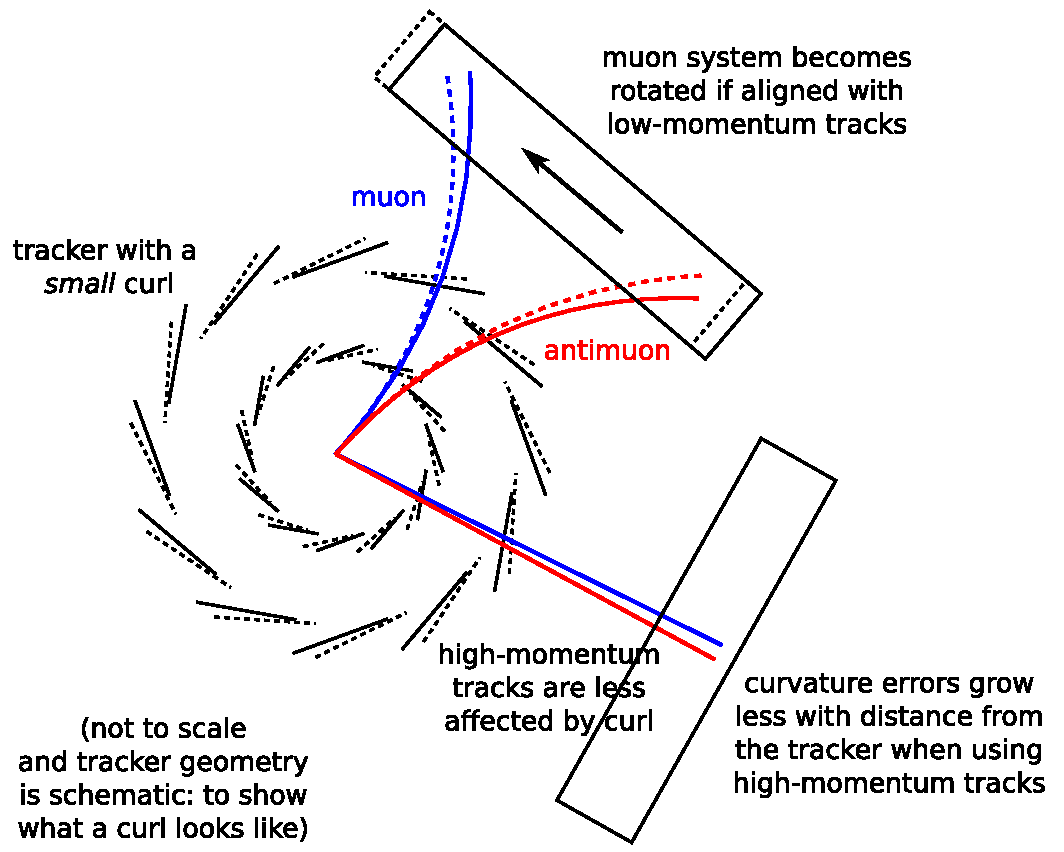
\includegraphics[width=\linewidth]{curl_explanation.pdf}
\end{frame}

\end{document}
